\section{Trial Wave Function}
An accurate trial wave function can drastically improve the accuracy of a variational QMC method such as VMC. Most highly accurate trial wave functions are entirely computationally intractable and are never implemented in QMC methods. In addition to being accurate and computationally tractable we seek for wave functions that satisfy known physical properties such as cluster decomposition as well as having an overall antisymmetry with respect to particle exchange due to nucleons obeying fermi statistics.

Cluster decomposition arises from the physical intuition that the wave function of two separate, non-interacting systems, $A$ and $B$ as in Figure~\ref{fig:cluster}, can be written as the product of their respective wave functions.
\begin{figure}[h]
   \centering
   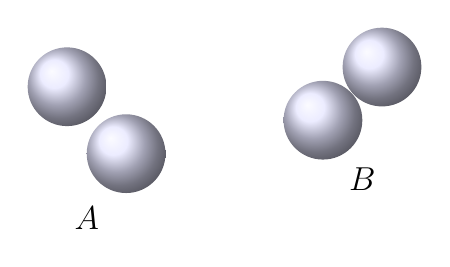
\begin{tikzpicture}[>=latex,scale=0.5]
      \shade[ball color=blue!10!] (-4.0,0.85) circle (1) ;
      \shade[ball color=blue!10!] (-2.5,-0.85) circle (1) ;
      \shade[ball color=blue!10!] (4.0,1.35) circle (1) ;
      \shade[ball color=blue!10!] (2.5,0.00) circle (1) ;
      \draw (-3.5,-2.5) node{\large $\ket{A}$};
      \draw (3.5,-1.5) node{\large $\ket{B}$};
   \end{tikzpicture}
   \caption{Two non interacting systems $A$ and $B$, whose composite wave function is the product $\ket{A+B}=\ket{A}\ket{B}$.}
   \label{fig:cluster}
\end{figure}
Mathematically this can be represented as a product of $n$-body functions, where $n$ is often 1 or 2 in our situation, though it could be higher. If a system is not cluster decomposable then unphysical correlations between non-interacting systems can occur.

The second property is that the wave function be antisymmetric overall. Since nucleons are fermions and the only degrees of freedom used in these calculations the product of different pieces of the wave function must be antisymmetric. Recent work in QMC has successfully included bosonic degrees of freedom such as pions \cite{madeira2018}, however that is not the case in this work.

%\begin{figure}[h!]
%   \centering
%   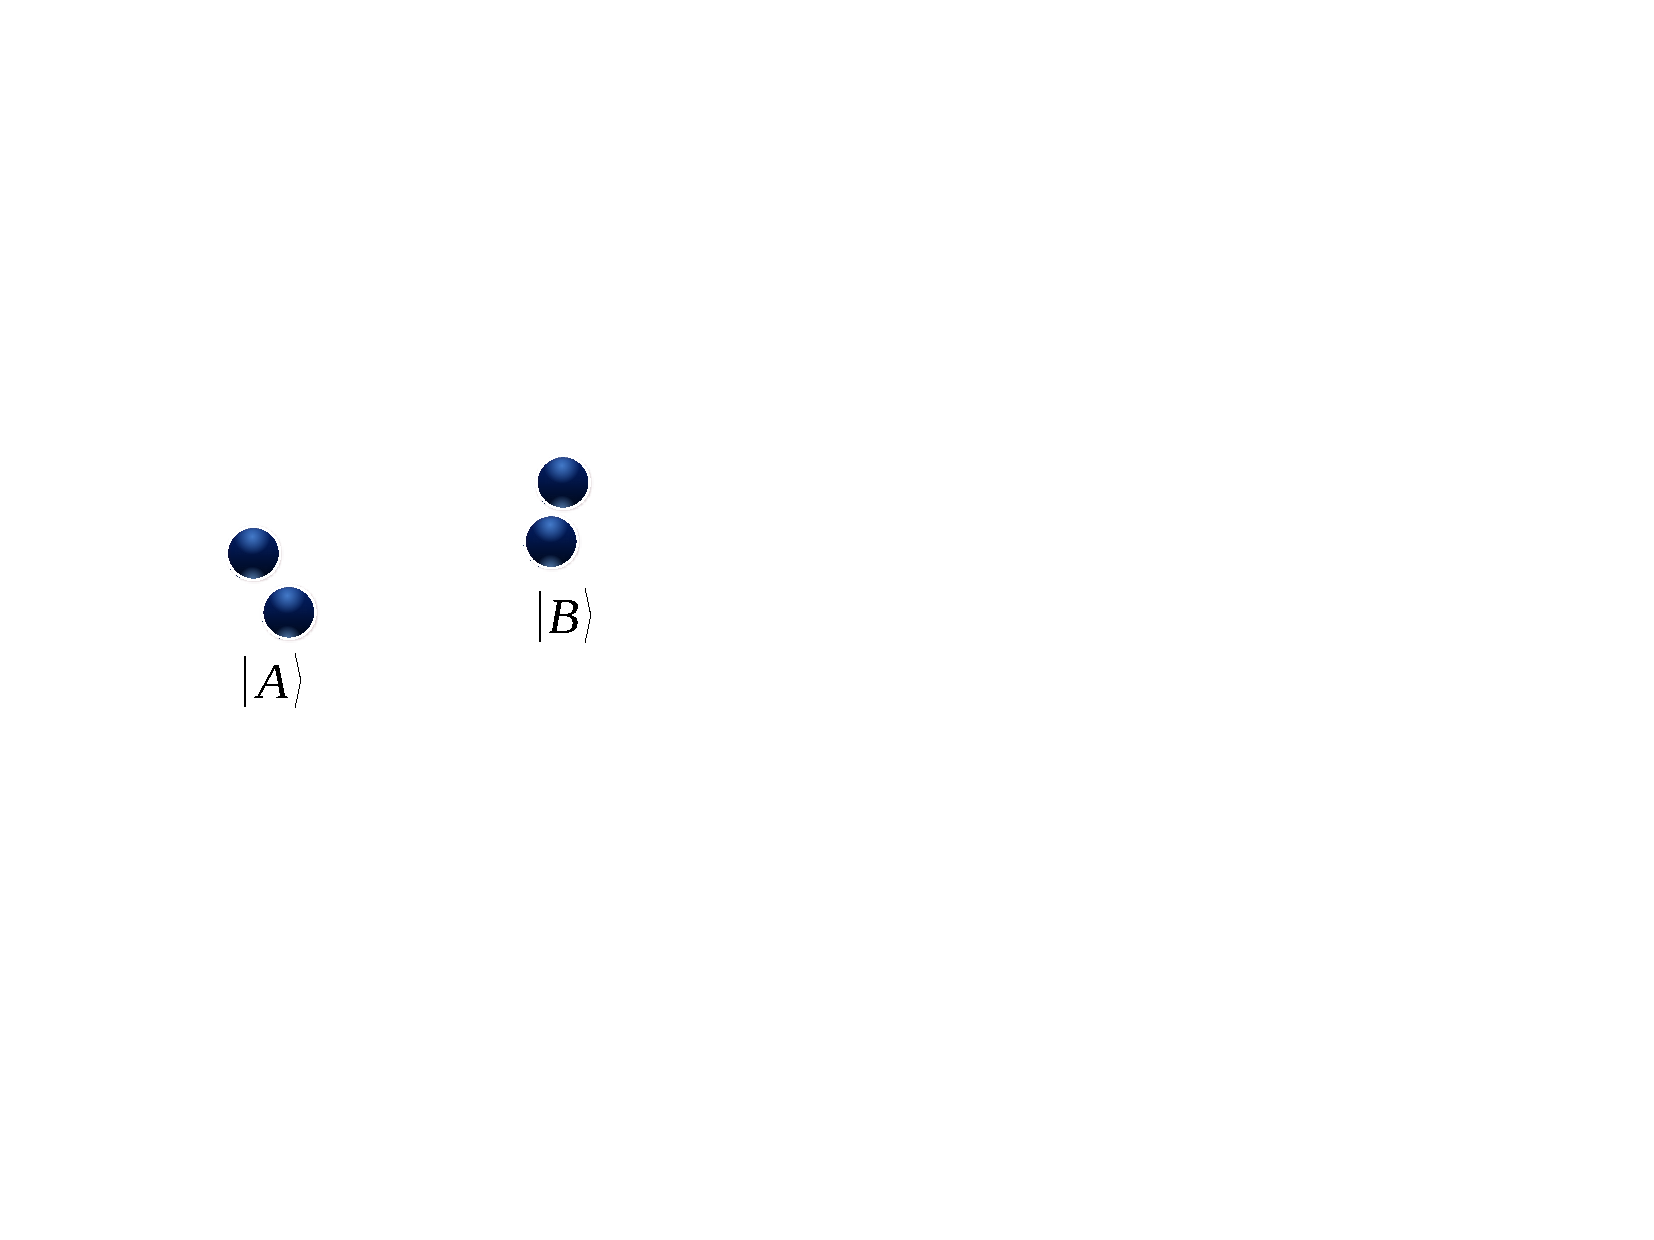
\includegraphics[width=\textwidth]{figures/cluster.pdf}
%   \caption{Energy per nucleon for ${}^4$He and ${}^{16}$O as calculated with linear, independent pair and quadratic correlations. Also, the energy per nucleon of symmetric nuclear matter of 28 particles in a periodic box with density $\rho=0.16$fm$^{-3}$. All calculations are compared to their expected values.}
%   \label{fig:cluster}
%\end{figure}

\subsection{Slater Determinant}
One of the simplest wave functions that satisfies the two properties specified above is the Slater determinant. The Slater determinant has been the starting place for a variety of many-body calculations in nuclear and condensed matter physics alike. In condensed matter the many-body wave functions will often be written in terms of a sum of weighted Slater determinants, where some methods have been able to use a sum of up to 2 billion determinants \cite{huron1973,li2018}. In nuclear physics a single determinant is often used for closed shell calculations and a sum of a small number, $\mathcal{O}(10)$, of weighted determinants is used for open shell systems. A Slater determinant is an antisymmetrized product of single particle (non-interacting) wave functions
\begin{equation}
   \Psi_{SD} = \mathcal{A} \left[\phi_1(\r_1)\phi_2(\r_2) \ldots \phi_A(\r_A)\right] =
   \begin{vmatrix}
      \phi_1(\r_1) & \phi_1(\r_2) & \ldots & \phi_1(\r_A) \\
      \phi_2(\r_1) & \phi_2(\r_2) & \ldots & \phi_2(\r_A) \\
      \vdots & \vdots & \ddots & \vdots \\
      \phi_K(\r_1) & \phi_K(\r_2) & \ldots & \phi_K(\r_A) \\
   \end{vmatrix},
\end{equation}
where the $\mathcal{A}$ is the antisymitrization operator and the $\phi_i(\r_j)$ are the overlap of the walker positions with the model single particle states. The single particle model states are made up of a radial and spin, iso-spin dependent parts,
\begin{equation}
   \phi_k = \Phi_{nj}\left[C_{c_l,m_s}^j Y_{l,m_l}(\hat{r}_i)\chi_s(s_i)\right]_{j,m_j},
\end{equation}
where $\Phi_{nj}$ is the radial part and the rest contains the spherical harmonics $Y_{l,m_l}(\hat{r}_I)$ and spin and iso-spin states where the Clebsch-Gordan coefficients ensure the correct $j$ and $m_j$ quantum numbers, and the different states are given by the index $k$. To accurately describe the wave function of an open shell nuclei each state with the correct total angular momentum and parity $J^\pi$ and isospin $T$ is included as a seperate Slater determinant.
\begin{equation}
   \braket{RS}{\Phi}_{J^\pi,T} = \sum\limits_n c_n D\{\phi_k(\r_i,s_i)\}
\end{equation}
Here the $c_n$ coefficients are variational parameters used to minimize the energy given a set of possible state configurations. One of the simplest examples of an open shell nuclei would be $^6$He whose ground state is a $J^\pi = 0^+$ state. The two protons and two of the neutrons could be in the full $(1S_{1/2})^2$ shell while the two remaining neutrons could be in the $(1P_{3/2})^2$ shell with their $m_j=\pm 3/2, \pm 1/2$ values being equal and opposite to ensure that $J=0$. This state has two possible determinants. Other possible configurations for the two remaining neutrons would be $(1P_{1/2})^2$ with one possible determinant, $(1D_{5/2})^2$ with three possible determinants, $(2S_{1/2})^2$ with one possible determinant and $(1D_{3/2})^2$ with two possible determinants giving a total of nine possible determinants. Notice that the two neutrons could be in a combination of $S$ and $D$ shells but never an $S$ and $P$ or $D$ and $P$ to ensure the parity of the state is positive. The number of determinants used for open shell nuclei will control how accurate the trial wave function is but for closed shell nuclei such as $^4$He or $^{16}$O a single slater determinant describing the full shell configuration is sufficient.

The radial part $\Phi_{nj}$ of the single particle states are obtained as bound state solutions to the single particle Schr\"odinger equation with a Woods-Saxon potential wine-bottle potential.
\begin{equation}
   v(r) = V_s\left[\frac{1}{1+e^{(r-r_s)/a_s}} + \alpha_se^{(-r/\rho_s)^2}\right]
\end{equation}
Here the parameters, $V_s, r_s, a_s, \alpha_s$ and $\rho_s$ are variational parameters used to shape the potential to obtain a minimum in energy.

%As an illustrative example consider the deuteron. The deuteron is in a iso-spin singlet state, $\frac{1}{\sqrt{2\pi}}(\ket{pn}-\ket{np})$. To show how the model state, $\ket{\Phi}$ would be built for this I will assume all entries are 1, though in practice the could all take on different numbers to account for the different spacial and spin dependencies of the state. Let's assume that both the neutron and the proton are in a spin up state. In this case the $\Phi(k,i)$ terms, where $k,i=1,2$, would take on the following values.
%\begin{align}
%   \phi(1,1)&=(1,0,0,0)=p\uparrow_1 \\
%   \phi(2,1)&=(0,0,1,0)=n\uparrow_1 \\
%   \phi(1,2)&=(1,0,0,0)=p\uparrow_2 \\
%   \phi(2,2)&=(0,0,1,0)=n\uparrow_2
%\end{align}
%The determinant of the Slater matrix can then be written as
%\begin{equation}
%\Psi_T=\det(S)=
%\begin{vmatrix}
%    \braket{k_1}{s_1} & \braket{k_1}{s_2} \\
%    \braket{k_2}{s_1} & \braket{k_2}{s_2}
%\end{vmatrix}
%=
%\begin{vmatrix}
%    p_1 & p_2 \\
%    n_1 & n_2
%\end{vmatrix}
%=
%p_1n_2-n_1p_2,
%\end{equation}
%which is the singlet state that we wanted to start with.

The Slater determinant is a mean-field wave function and is often used with Jastrow type short range correlations.
\begin{equation}
   \braket{RS}{\psi_T} = \bra{RS}\prod\limits_{i<j}f(r_{ij}) \ket{\phi}
\end{equation}
These correlations are spin-isospin independent and depend only on the particle separation and improve upon the uncorrelated Slater determinant wave function significantly. To maintain the cluster decomposition the functions $f(r_{ij})$ must go to unity for large particle seperations. In this work we have used Slater determinant wave functions with a Jastrow factor and spin-isospin dependent correlations which will be discussed in a later section. \red{ADD PLOT AND CITATION BACKING THIS CLAIM HERE}.

\subsection{Pfaffian Wave Function}
Another wave function that obeys these properties is the paired Pfaffian wave function. This wave function was developed to describe Cooper pairs which form when, at low temperature, paired fermions, such as electrons or $^3$He, are energetically favorable to free particles. 
\red{Explain what it is.}
\red{\\ Explain why it's useful.}

\subsection{Spin-Isospin Dependent Correlations}
\red{Explain what properties you need, etc.}

\subsubsection{Quadratic Correlations}
\red{Be sure to include results}

\subsubsection{Exponential Correlations}
\red{Why aren't they working}

\subsubsection{Alessandro's correlations and $T^2$ fix to them - \red{Maybe just do $T^2$ fix and apply it to exponential correlations}}
